% file: graph-decomposition/tree.tex

\documentclass[tikz]{standalone}
\usepackage{tikz-qtree}

\begin{document}
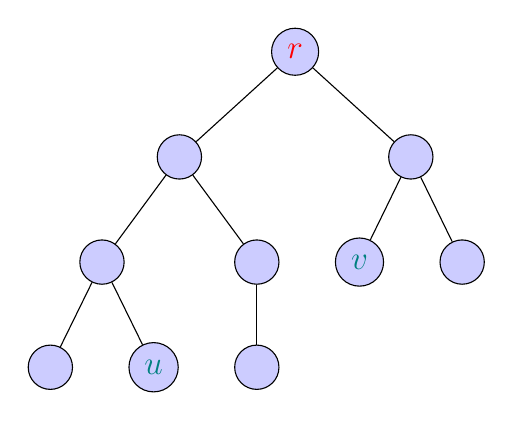
\begin{tikzpicture} [level distance = 38pt, sibling distance = 20pt,
  edge from parent/.style= { % added code
      draw, edge from parent path = {(\tikzparentnode) -- (\tikzchildnode)}}]
  \tikzset{every tree node/.style = 
    {align = center, circle, draw, fill = blue!20, font = \large, minimum size = 16pt}}
    \Tree [.\textcolor{red}{$r$}
	    [.$$
	       [.$$ 
		$$
		\textcolor{teal}{$u$}
	       ]
	       [.$$
		$$
	       ]
            ]
	    [.$$ 
	      [.\textcolor{teal}{$v$} ]
	      $$
	   ] 
        ]
\end{tikzpicture}
\end{document}
